\section{Observaciones}

\begin{figure}[htbp]
	\centering
	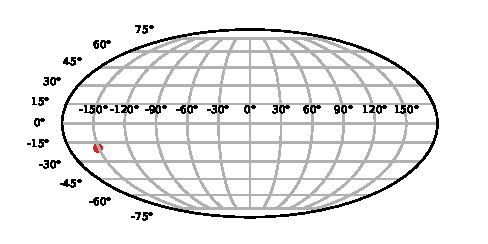
\includegraphics{lb.pdf}
	\caption{Coordenadas galácticas}
	\label{fig:lb}
\end{figure}

\begin{figure}[htbp]
	\centering
	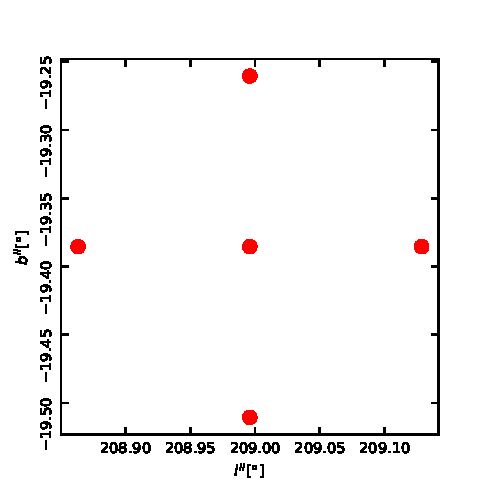
\includegraphics{cruz.pdf}
	\caption{Cruz de observación}
	\label{fig:cruz}
\end{figure}

\begin{figure}[htbp]
	\centering
	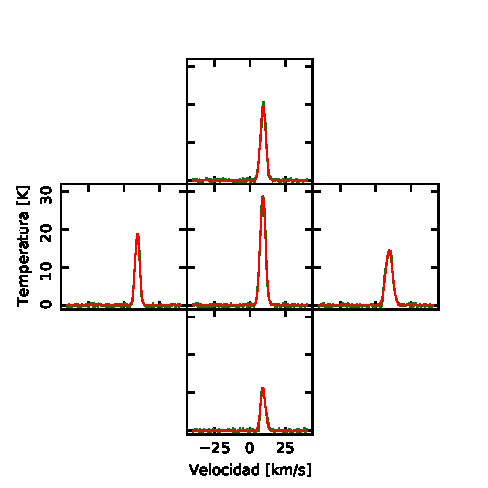
\includegraphics{specfit1.pdf}
	\caption{Ajuste gaussiano 1}
	\label{fig:specfit1}
\end{figure}

\begin{figure}[htbp]
	\centering
	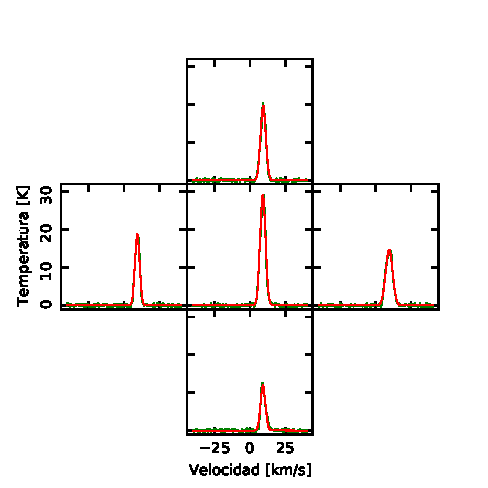
\includegraphics{specfit2.pdf}
	\caption{Ajuste gaussiano 2}
	\label{fig:specfit2}
\end{figure}

\begin{figure}[htbp]
	\centering
	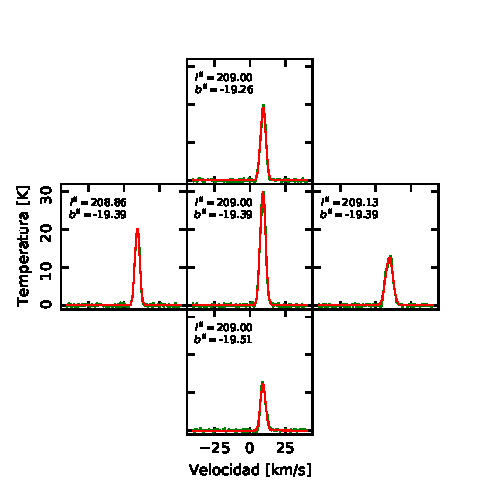
\includegraphics{specfit3.pdf}
	\caption{Ajuste gaussiano 3}
	\label{fig:specfit3}
\end{figure}

\begin{figure}[htbp]
	\centering
	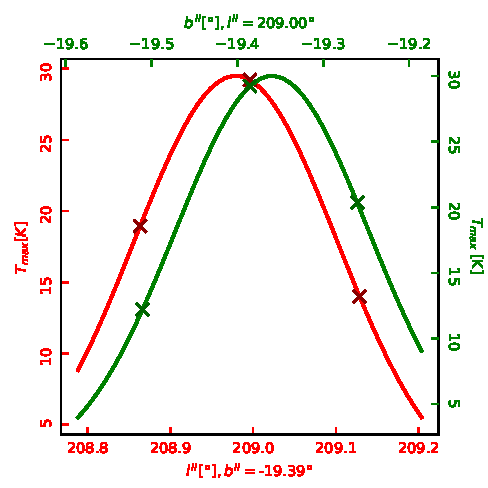
\includegraphics{tmax.pdf}
	\caption{Ajusta gaussiano de temperatura máxima}
	\label{fig:tmax}
\end{figure}

\begin{figure}[htbp]
	\centering
	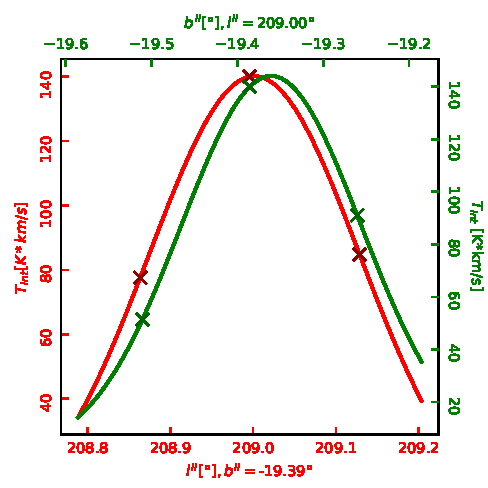
\includegraphics{tint.pdf}
	\caption{Ajuste gaussiano de temperatura integrada}
	\label{fig:tint}
\end{figure}